\documentclass[11pt, a4paper]{article}
\usepackage{graphicx} % Required for inserting images
\usepackage{caption} % for captions
\usepackage{bbm} % Math font; use \mathbbm{}
\usepackage[acronym]{glossaries} % for acronyms
\usepackage{physics} % Physics symbols

\usepackage{showlabels} % To show equations labels on the PDF. Comment at the end

% Defining acronyms
\newacronym{etk}{ETK}{Einstein Toolkit}

% Defining variables
\newcommand\figifcap{Initial and final conditions}

\title{Numerical Relativity Homework 2}
\author{Federico Leto di Priolo}
\date{June 2024}

\begin{document}

\maketitle

\section{Sod Shock Tube Problem}

The Sod shock tube problem consists in a one-dimensional Riemann
problem with Initial discontinuities in density and pressure. The time
evolution of the system can be computed by solving the Euler equations.
Since the solution of this problem can be computed exactly, it is useful
to test the accuracy of numerical codes. In this exercise we solve the
Sod problem with the \acrfull{etk} using different resolutions and we
compare the results with the exacts solution.

The solution to the problem is described by three characteristics, each
of them related to the propagation speed of the fluid in different
regions. Those can be associated to either a rarefaction wave, a shock
wave, or a contact discontinuity. Specifically, the pressure and the
velocity of the fluid develops a rarefaction wave and a shock wave, while
the density develops also a contact discontinuity. The exact solution
along with the initial conditions is shown in Figure
\ref{fig:all_exact_if}.

For the numerical solutions the HLLE Riemann solver has been used, along
with the Minmod slope limiter. The domain extends in the range
\([-0.5, 0.5]\) and the evolutions proceeds up to time \(t = 0.4\).
The used grid spacing are \(\{0.005, 0.0025, 0.00125, 0.000625\}\),
corresponding respectively to \(\{200, 400, 800, 1600\}\) grid points.

\subsection{Higher Resolution: 1600 points}

We will use the results obtained with the highest resolutions to showcase
how the numerical solutions look like. Figure
\ref{fig:all_1600_snapshots} shows some snapshots of the profiles of
density, pressure and velocity of the fluid, including the initial and
the final ones. As can be seen, S and CD waves travel in opposite
direction with respect to the R waves. We point out that the fact that
the initial profile in Figure \ref{fig:all_1600_snapshots} doesn't
perfectly resemble a step (as it should) is just due to the way the
numerical results are interpolated on the chosen uniform grid
\([-0.45, 0.45]\). Figure \ref{fig:all_1600_initial_compare} compares
the interpolated initial data along with the raw initial data actually
used by the \acrshort{etk}.

\begin{center}
    \centering
    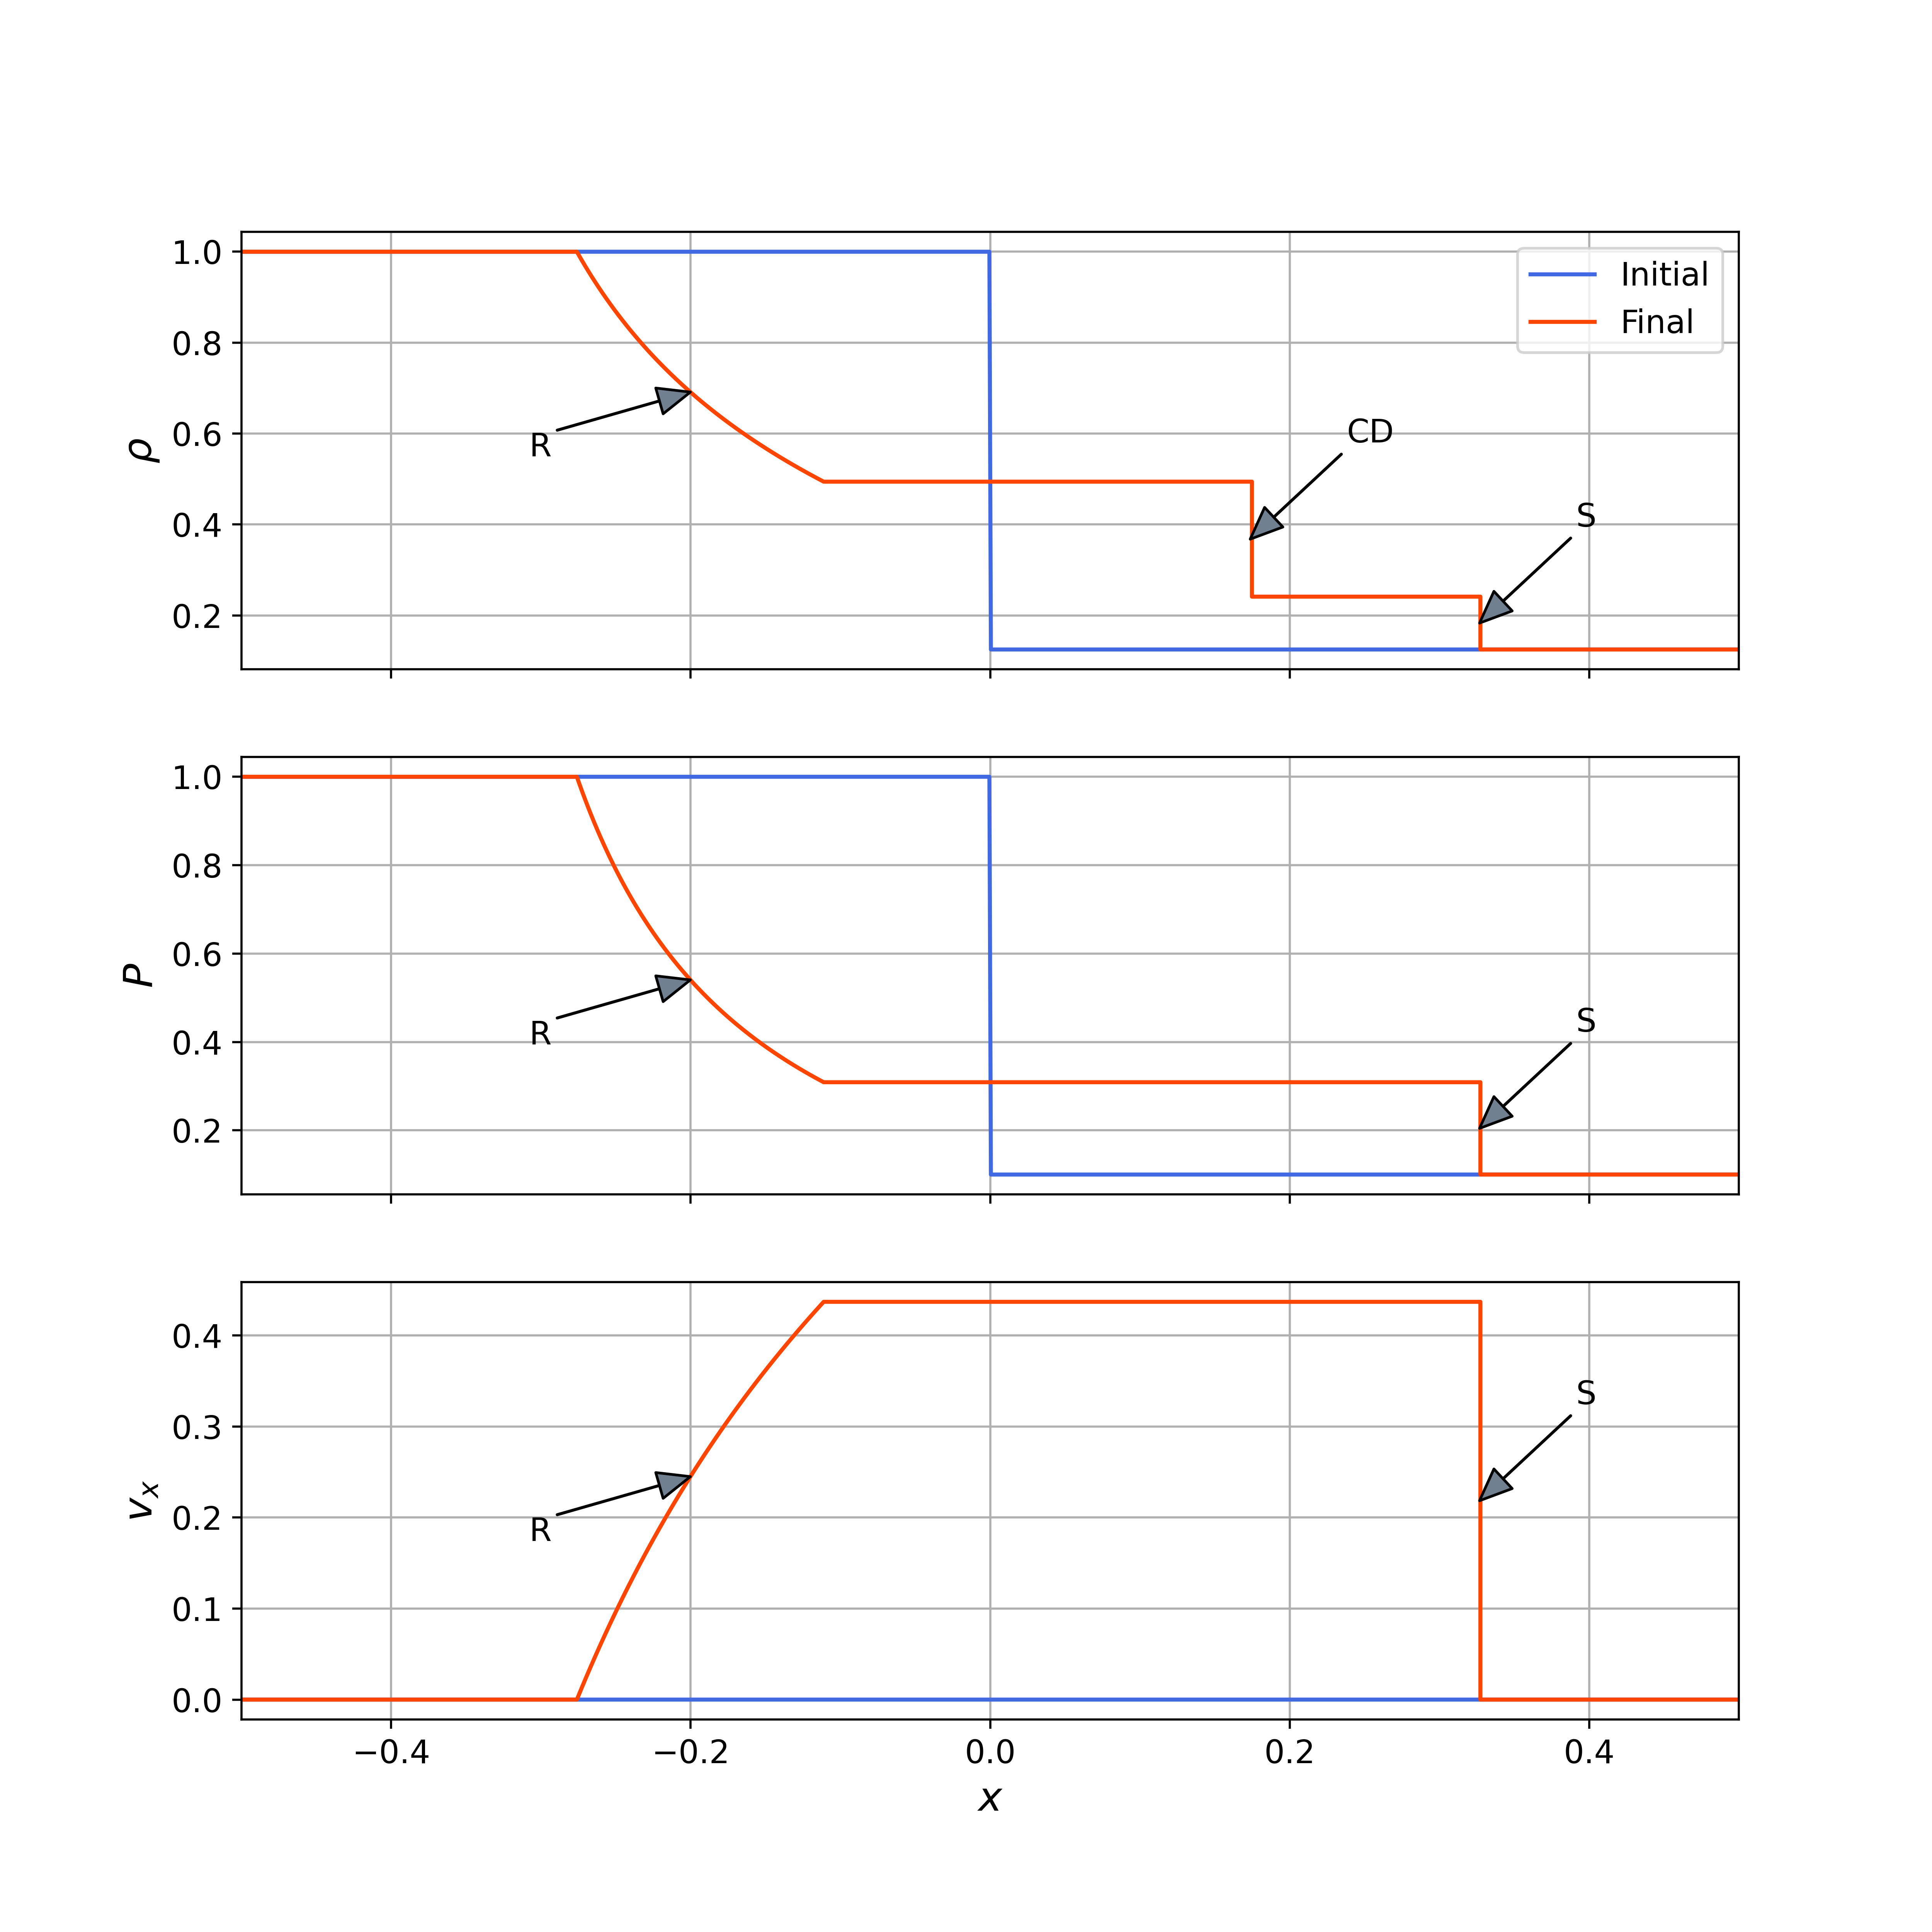
\includegraphics[width=1\linewidth]{images/all_exact_if.png}
    \captionof{figure}{Exact Solution; \figifcap; The arrows points at the different types of waves: R (Rarefaction), S (Shock) and CD (Contact Discontinuity).}
    \label{fig:all_exact_if}
\end{center}

\begin{center}
    \centering
    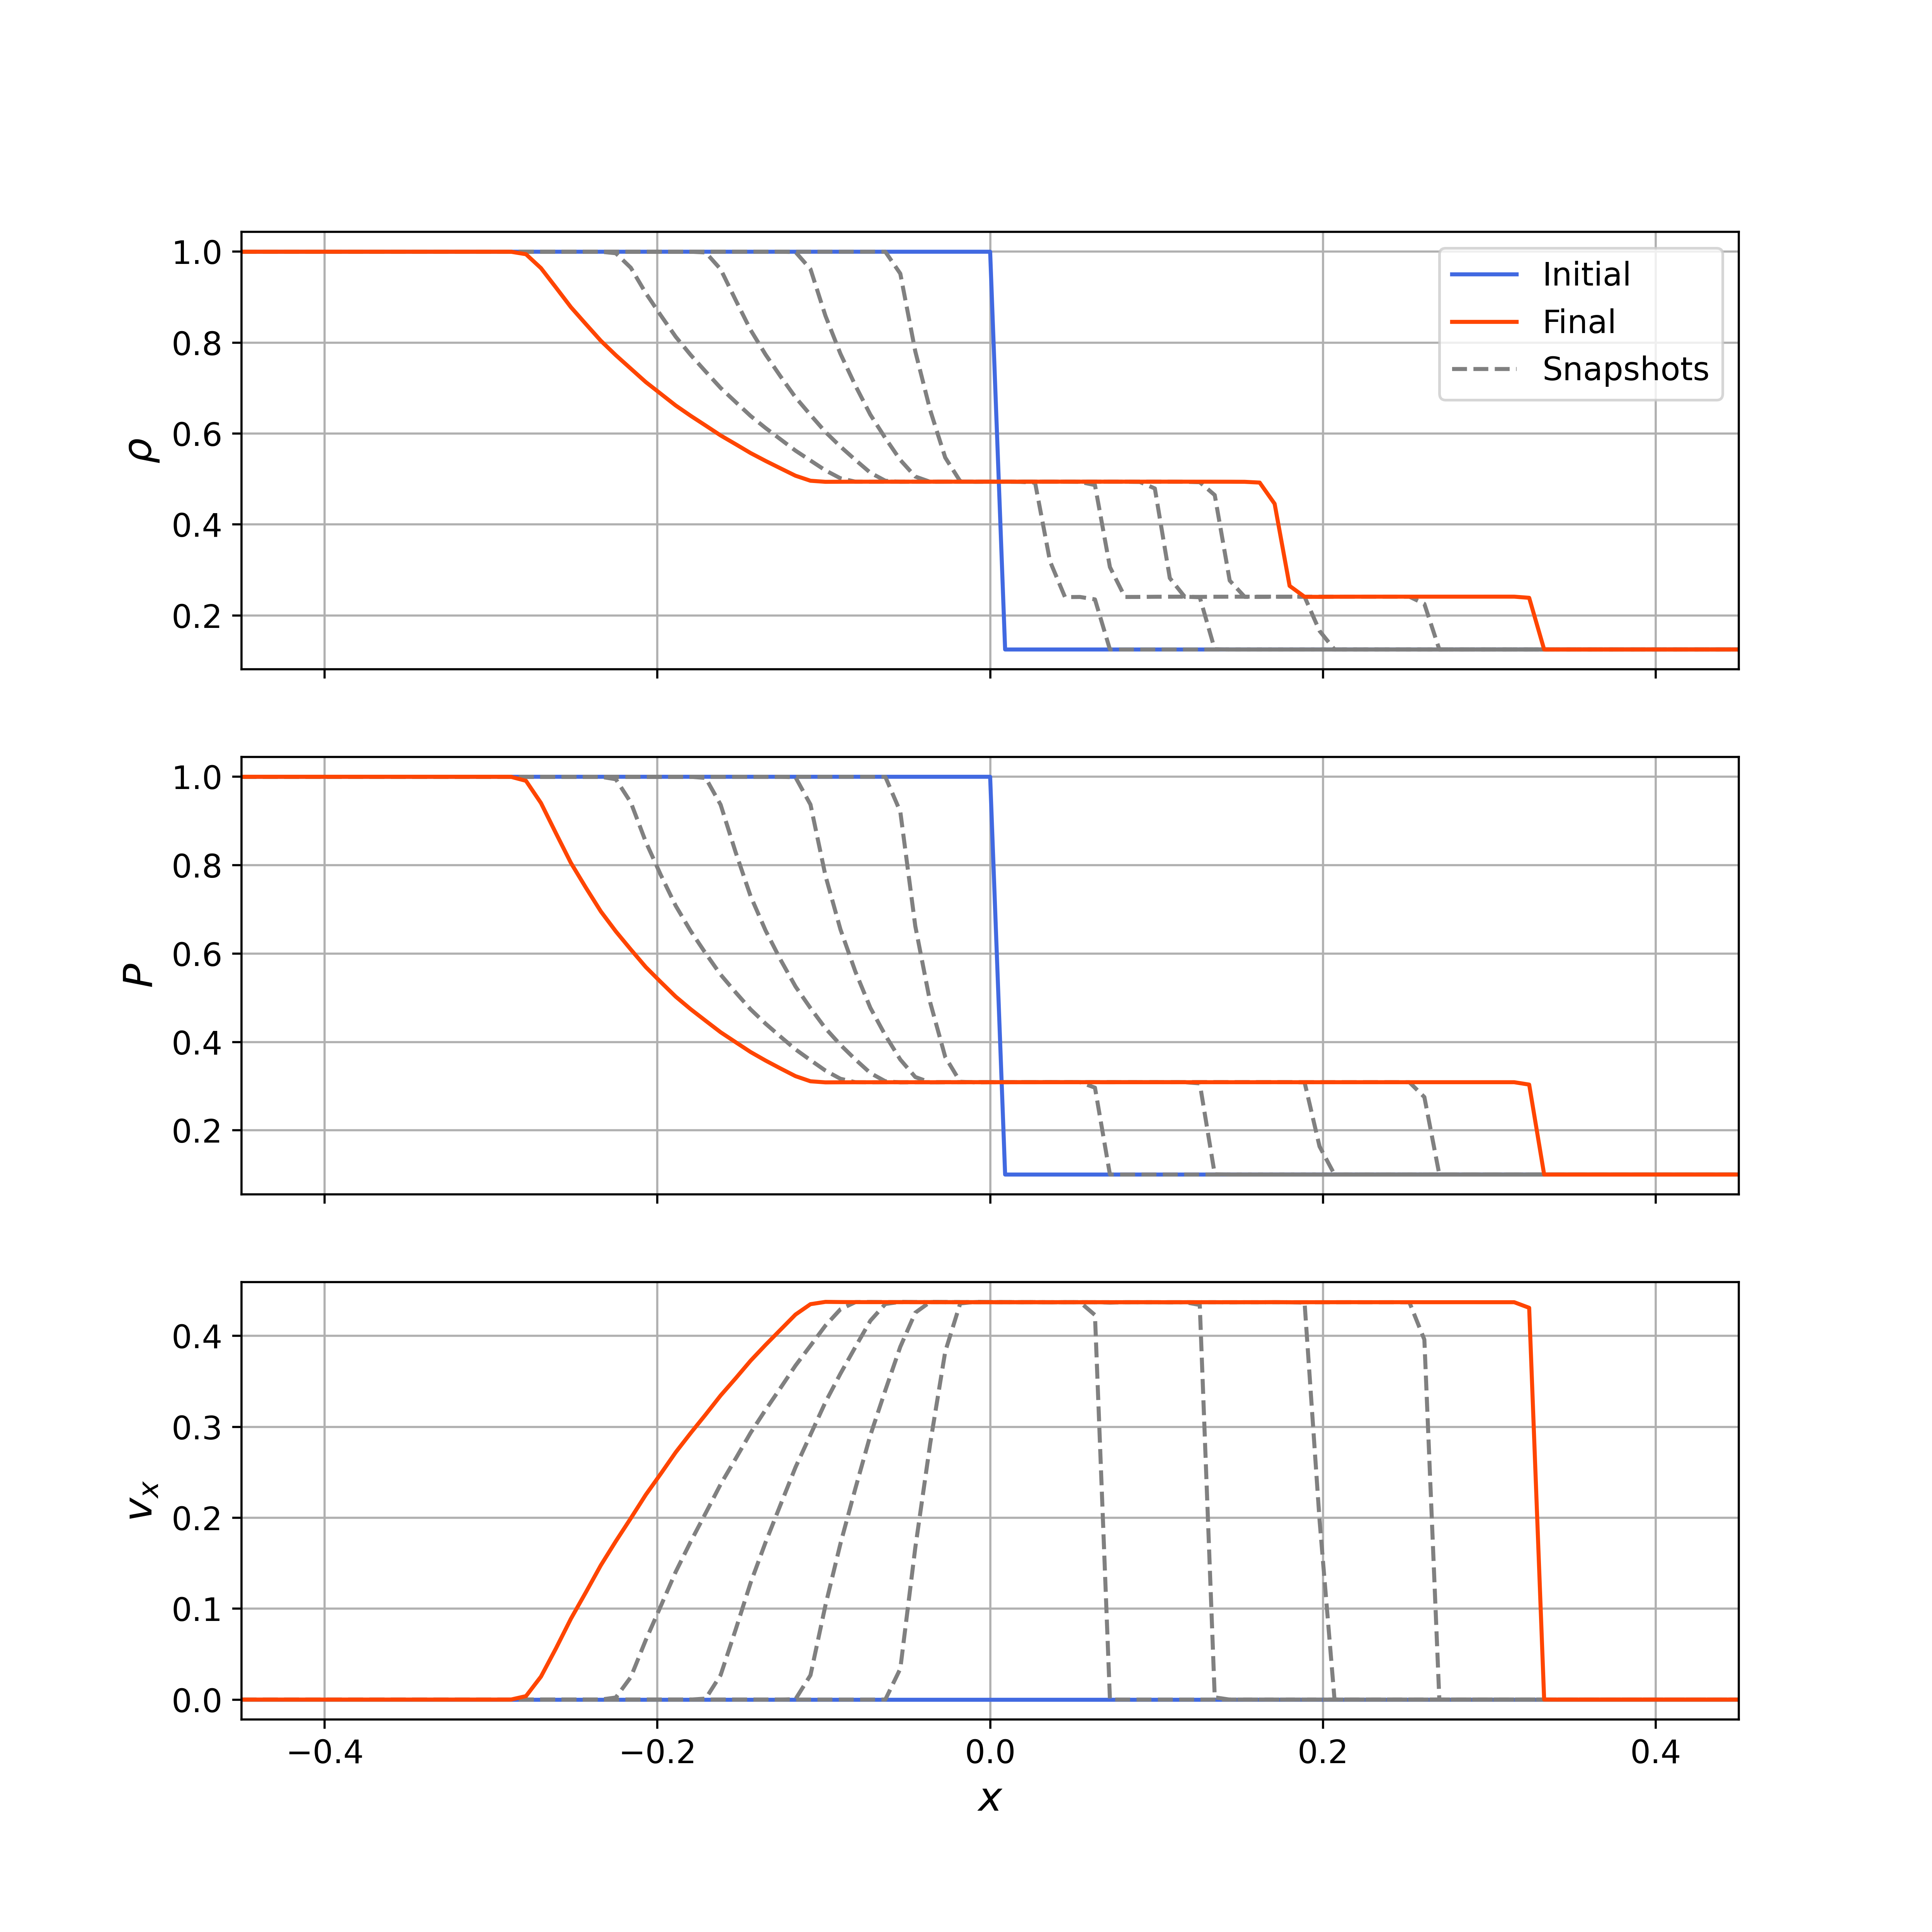
\includegraphics[width=1\linewidth]{images/all_1600_snapshots.png}
    \captionof{figure}{Numerical Solution; 1600 points; Snapshots.}
    \label{fig:all_1600_snapshots}
\end{center}

\begin{center}
    \centering
    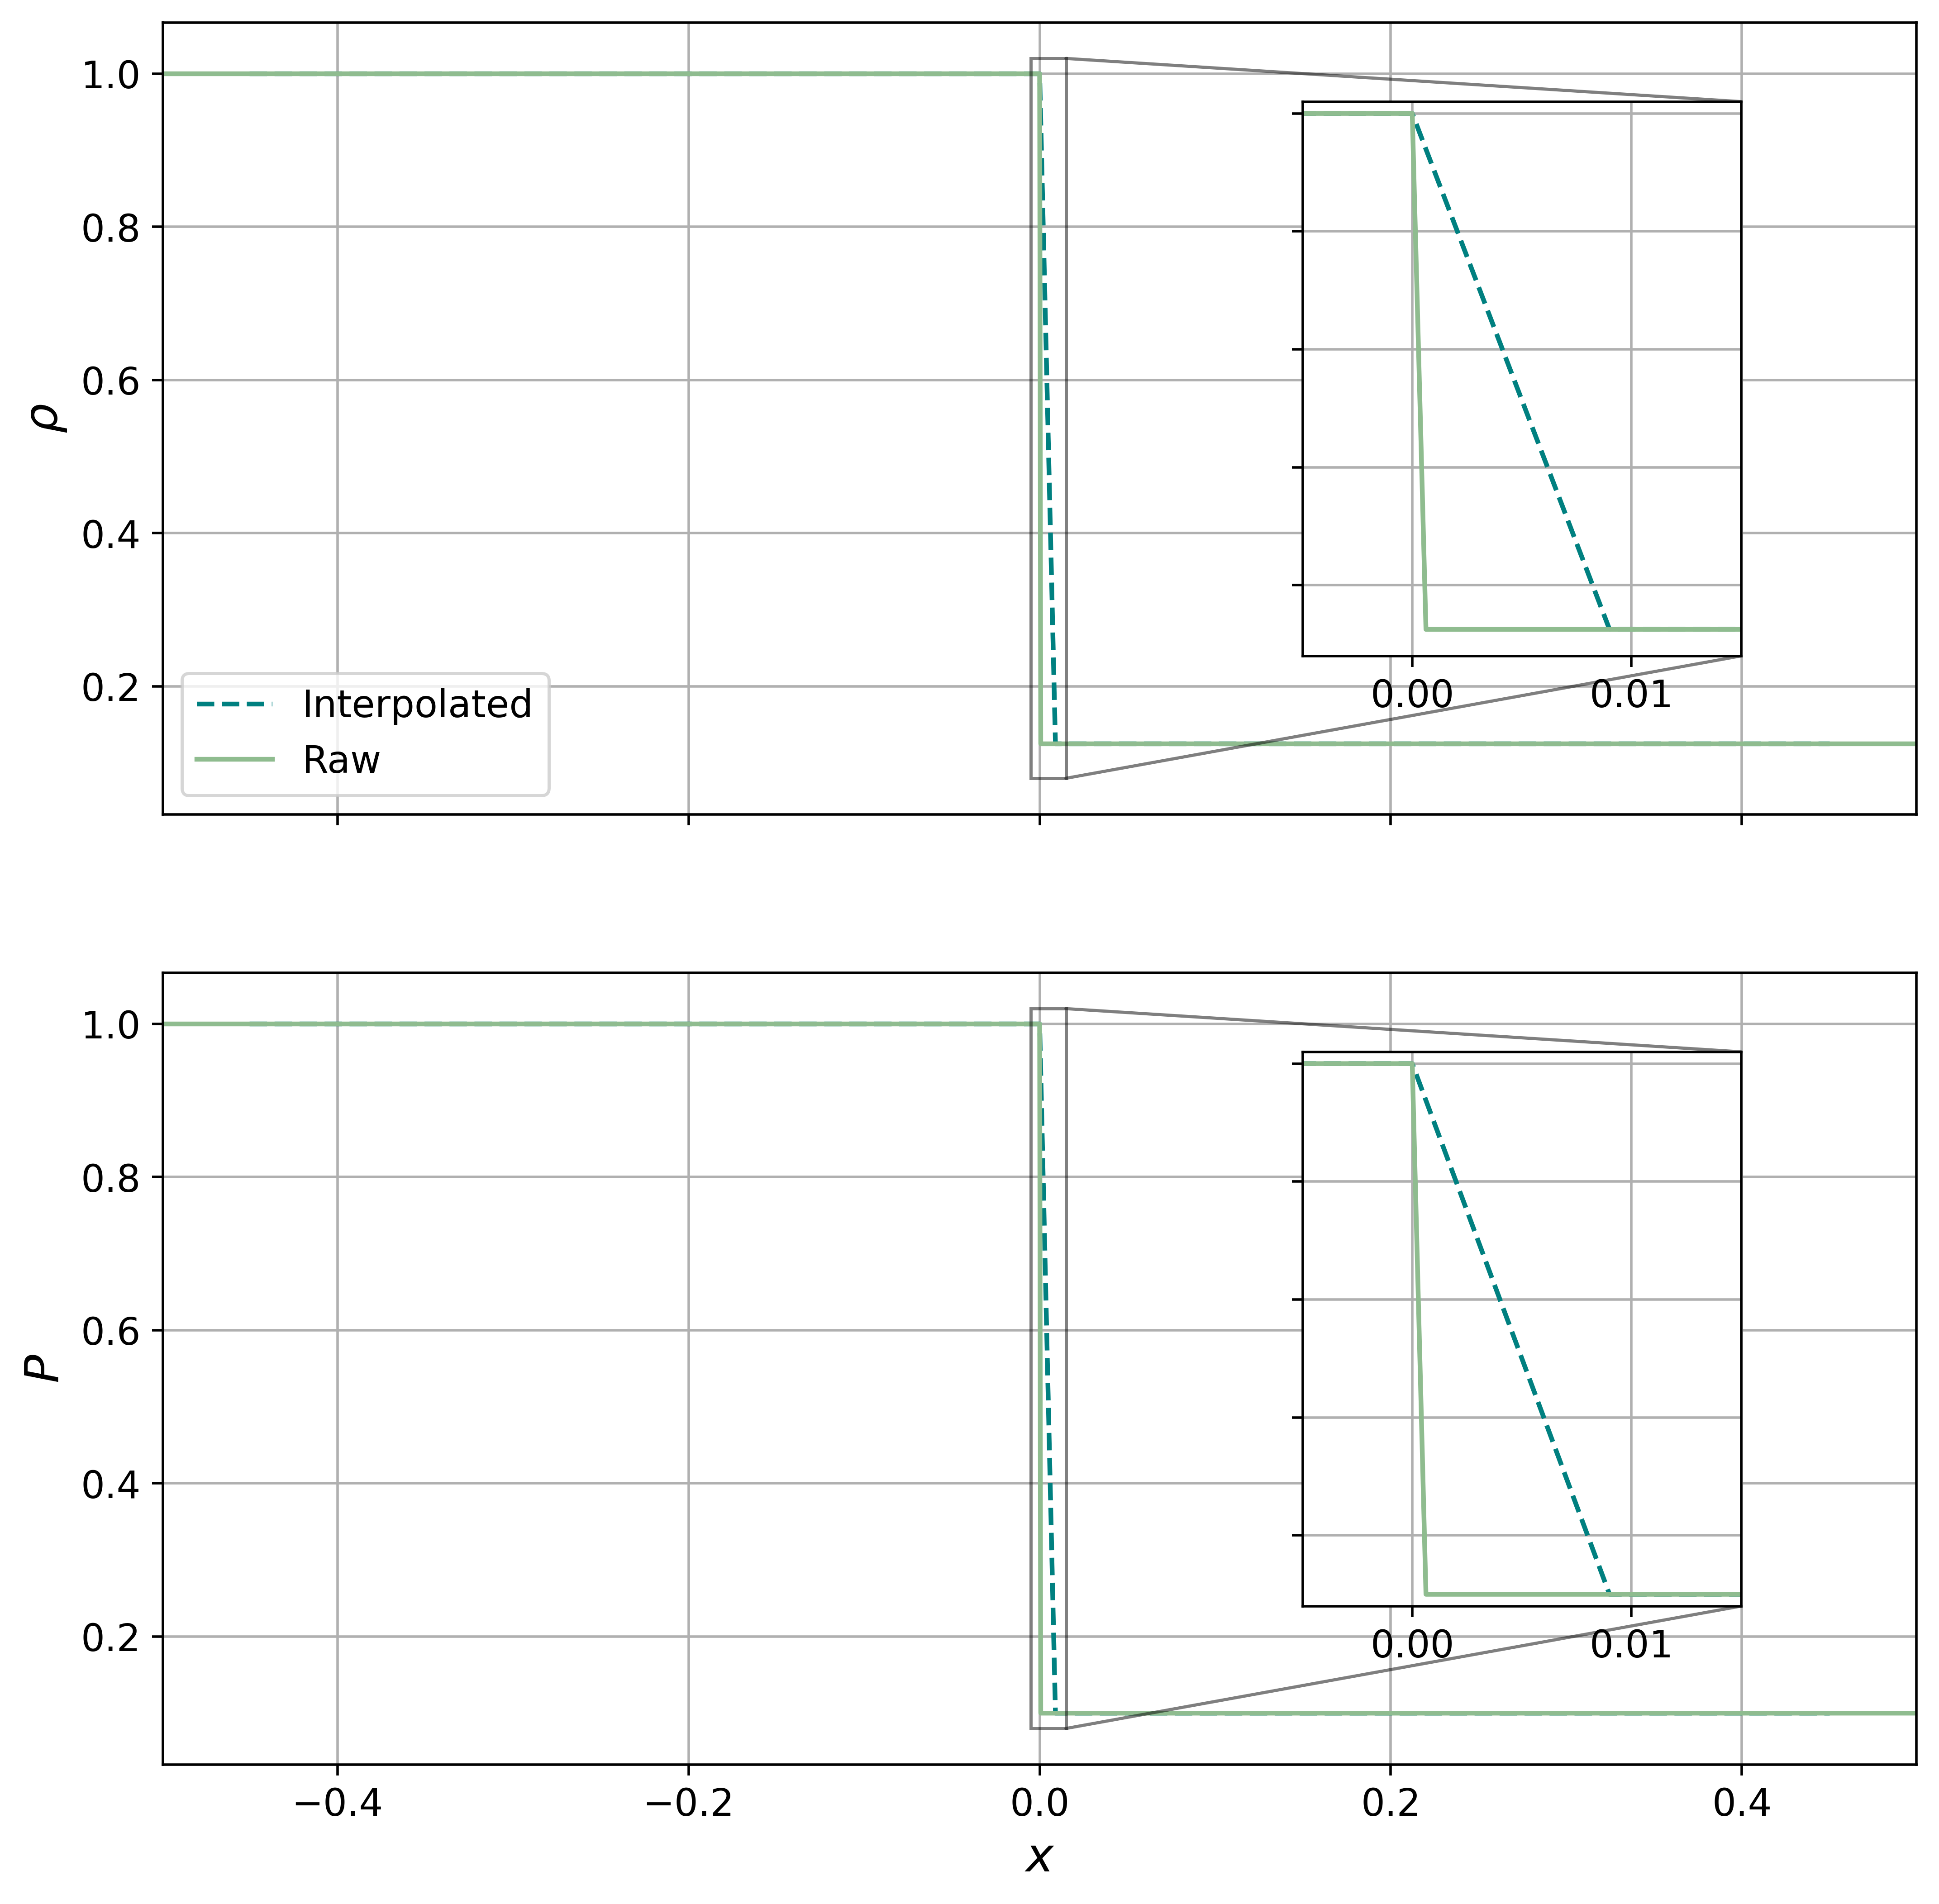
\includegraphics[width=1\linewidth]{images/all_1600_initial_compare.png}
    \captionof{figure}{Initial data; 1600 points; Raw and interpolated.}
    \label{fig:all_1600_initial_compare}
\end{center}

\end{document}
